% !TEX encoding = UTF-8 Unicode 

\section{Development approaches}

The definition of mobile development can be more or less general. It can be seen as a broad process of implementing a mobile application starting with planning and designing and finishing with testing and releasing. A more software-oriented definition is that mobile development simply refers to implementing an application for mobile devices by coding it using a selected technology stack \cite{microsoft_mobile_development}.

Mobile development can become a complex task considering the variety of devices and platforms available on the market. There are many different approaches available and in order to choose one over another the mobile application requirements should be taken into account as well as target platforms and devices, development and time costs \cite{velvetech_mobile_dev_approaches}.

In this chapter, there are presented selected popular approaches to mobile application development. Each of them is described mainly in the context of architecture, technology stack and tools, platforms supported and possible advantages or disadvantages.

\subsection{Native mobile development}

Since almost a decade, the mobile operating system market has been dominated by Android and iOS, reaching 99,3\% in March 2023 \cite{statcounter_mobile_os_market}. For this reason, in the context of this thesis only the above mentioned operating systems are being taken into account.

Native mobile development encompasses building mobile applications that can only be implemented using a platform-specific programming language and deployed to a single operating system \cite{comparative_analysis_native_hybrid}. Such an approach brings with it the necessity for creating and maintaining multiple codebases and with that possibly multiple development teams \cite{approach_to_assess_performance_case_study}. The number of distinct codebases does is not simply equal to the number of target platforms as different versions of a single platform may require to be implemented independently. 

\begin{figure}[H]
    \begin{minipage}{.47\textwidth}
      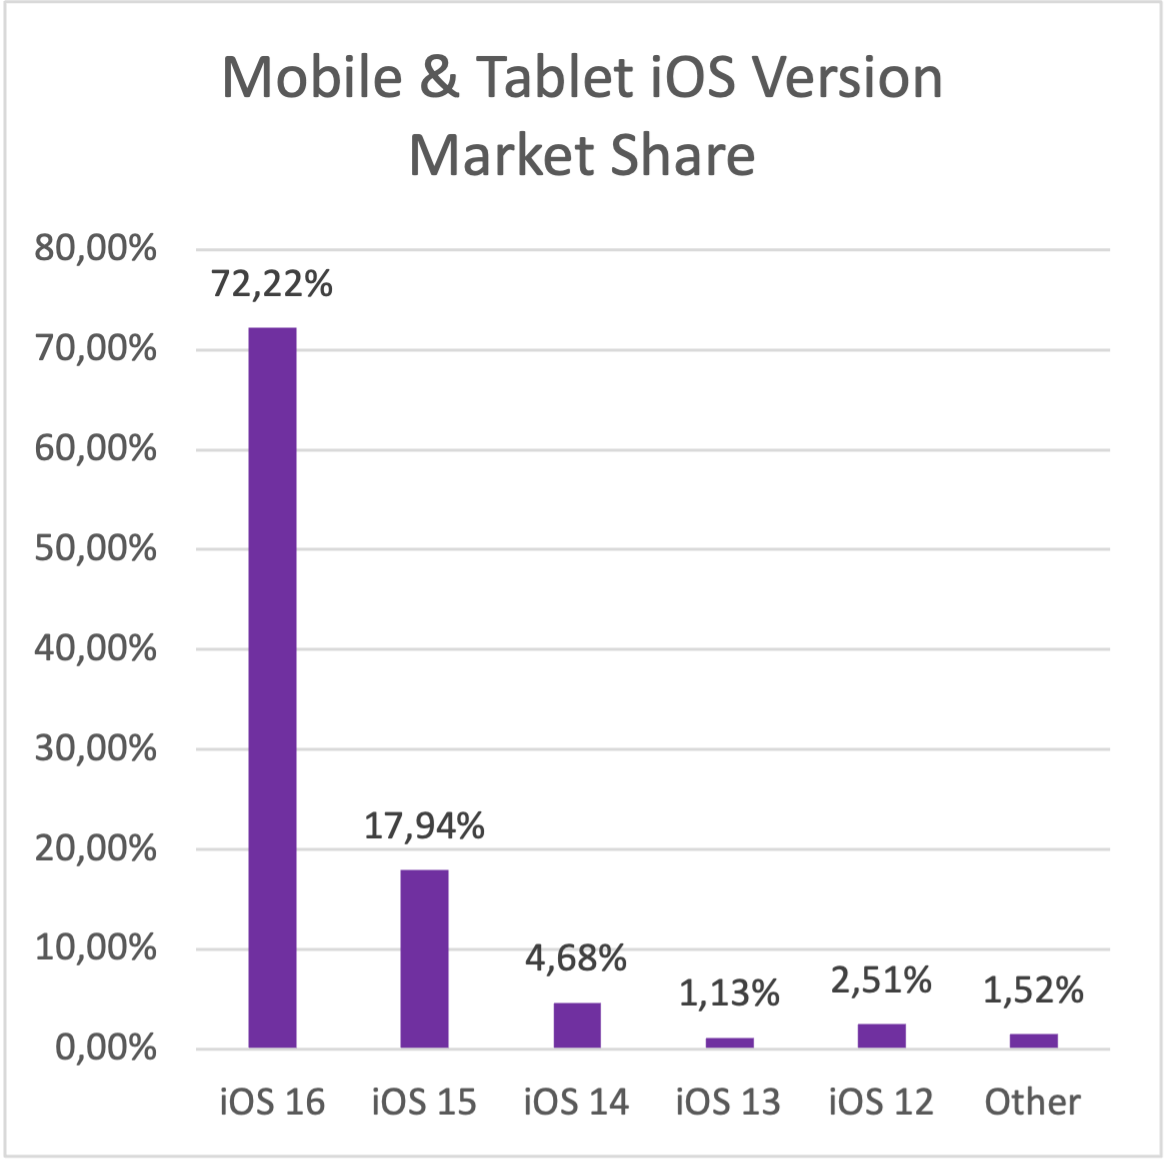
\includegraphics[width=\textwidth]{img/ios_ver_market_share}
      \caption{iOS version market share \cite{statcounter_ios_version_market}}
      \label{fig:ios_versions}
    \end{minipage}
    \hfill
    \begin{minipage}{.47\textwidth}
      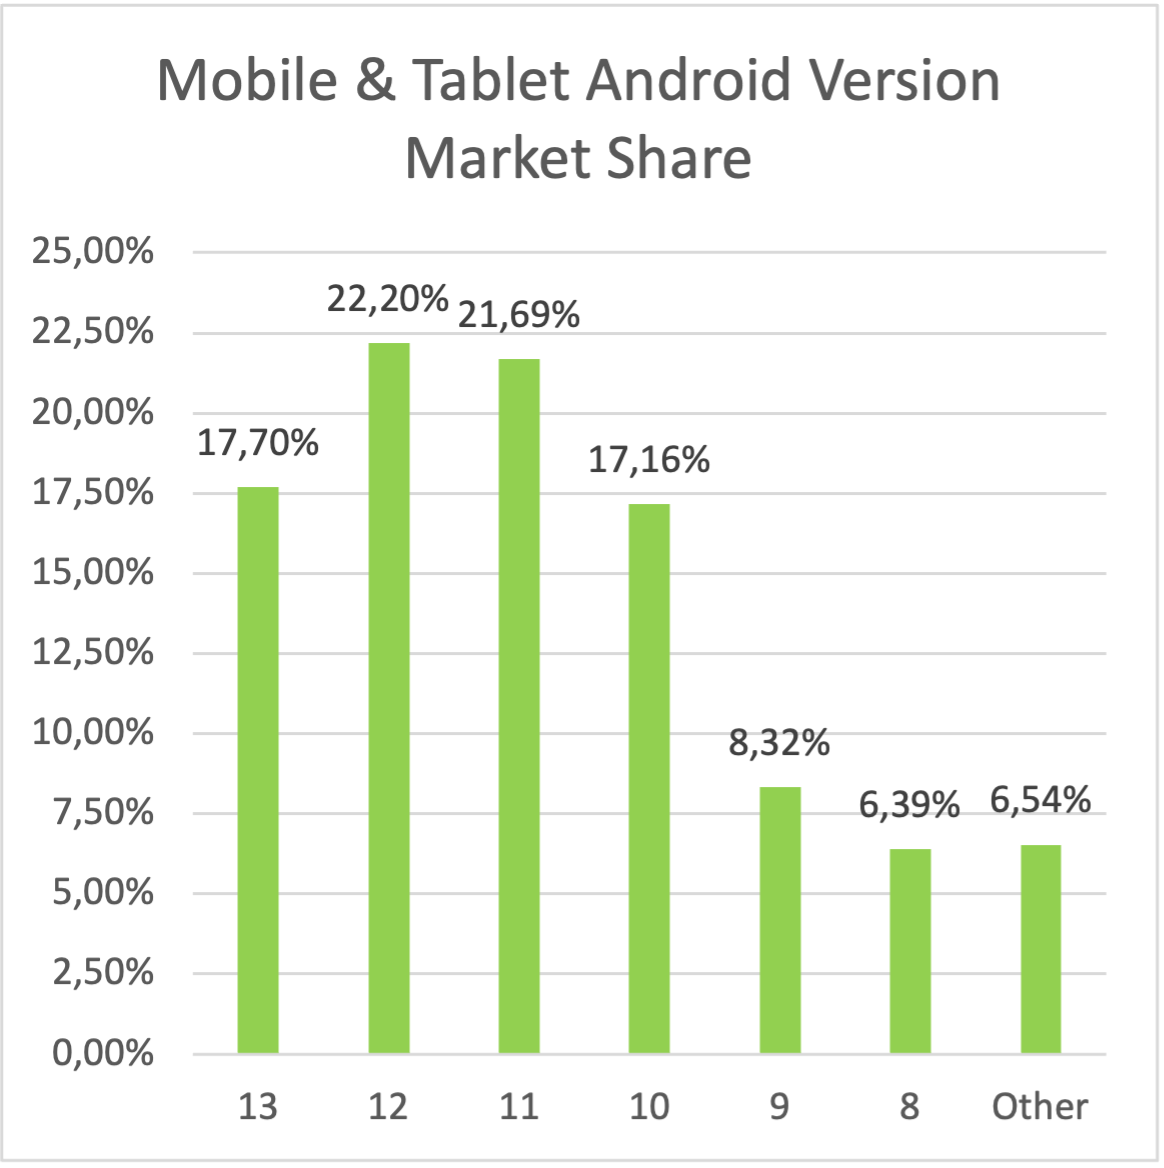
\includegraphics[width=\textwidth]{img/android_ver_market_share}
      \caption{Android version market share \cite{statcounter_android_version_market}}
      \label{fig:android_versions}
    \end{minipage}
\end{figure}

As can be seen in the Figure \ref{fig:ios_versions}, in case of iOS, almost 90\% of devices are running either the most or second-most recent major version of the operating system. Therefore, when targeting the Apple's system, probably a single codebase would be enough.

However, in case of Android, there is a high level of market fragmentation, as nearly 20\% of smarthones or tablets are running older versions released as far as in 2015 (Figure \ref{fig:android_versions}). Because there are limitations such as deprecation of code commands and API bahavior changes between distant versions, multiple codebases may be chosen to be maintained separately per a single mobile application.

\subsubsection{Android}
Include Material!!!

\subsubsection{iOS}
Include Cupertino!!!